\documentclass[border = 1mm]{standalone}

%cool packages
\usepackage[utf8]{inputenc}% That awesome utf8 characters
\usepackage[T1]{fontenc}% Those nice fonts
\usepackage{mathtools,amssymb,bm} %math
\usepackage{siunitx} % typesetting for units
\usepackage[draft,margin]{fixme} % for notes, remove draft if final version
\usepackage{graphicx} % for inserting figures
\usepackage{acronym} %for having acronyms
\usepackage{tikz} % for drawing stuff
\usepackage{pgfplots} %for plotting data or math functions
\usepackage{xcolor} % for having nicer colours
\usepackage{ifthen} % boolean checks

%penalties for having clubs or widows
\clubpenalty10000 
\widowpenalty10000

%cool memoir stuff
%The cool memoir stuff is wrapped in a check. This is done to see if the document class actually supports it.

\makeatletter%
\@ifclassloaded{memoir}%
  {%
\newsubfloat{figure} %allowing sub figures
\graphicspath{{./figures/}{../figures/}} % no need for those pesky folder extensions in the actual file
  }%
  {}%
\makeatother%

% new commands

\newcommand\numberthis{\addtocounter{equation}{1}\tag{\theequation}} %numbering equations in align* or aligned*

%\newcommand{colourscheme}[1]%
%{%
%        \ifthenelse{\eqal{#1}{1}}{%       
%                \definecolor{c1}{rgb}{0,0,0}
%                \definecolor{c2}{rgb}{0,0,0}
%                \definecolor{c3}{rgb}{0,0,0}
%                \definecolor{c4}{rgb}{0,0,0}
%                \definecolor{c5}{rgb}{0,0,0}
%                \definecolor{c6}{rgb}{0,0,0}
%                \definecolor{c7}{rgb}{0,0,0}
%                \definecolor{c8}{rgb}{0,0,0}
%                \definecolor{c9}{rgb}{0,0,0}
%                \definecolor{c10}{rgb}{0,0,0}
%                \definecolor{c11}{rgb}{0,0,0}
%                \definecolor{c12}{rgb}{0,0,0}
%                \definecolor{c13}{rgb}{0,0,0}
%                \definecolor{c14}{rgb}{0,0,0}
%                \definecolor{c15}{rgb}{0,0,0}
%                \definecolor{c16}{rgb}{0,0,0}
%        }%
%        {}%
%        \ifthenelse{\eqal{#1}{2}}{%       
%                \definecolor{c1}{rgb}{0,0,0}
%                \definecolor{c2}{rgb}{0,0,0}
%                \definecolor{c3}{rgb}{0,0,0}
%                \definecolor{c4}{rgb}{0,0,0}
%                \definecolor{c5}{rgb}{0,0,0}
%                \definecolor{c6}{rgb}{0,0,0}
%                \definecolor{c7}{rgb}{0,0,0}
%                \definecolor{c8}{rgb}{0,0,0}
%                \definecolor{c9}{rgb}{0,0,0}
%                \definecolor{c10}{rgb}{0,0,0}
%                \definecolor{c11}{rgb}{0,0,0}
%                \definecolor{c12}{rgb}{0,0,0}
%                \definecolor{c13}{rgb}{0,0,0}
%                \definecolor{c14}{rgb}{0,0,0}
%                \definecolor{c15}{rgb}{0,0,0}
%                \definecolor{c16}{rgb}{0,0,0}
%        }%
%        {}%
%} % this command creates some colours, based on the input. 

\definecolor{c1}{rgb}{0,0,0}
\definecolor{c2}{rgb}{0,0,0}
\definecolor{c3}{rgb}{0,0,0}
\definecolor{c4}{rgb}{0,0,0}
\definecolor{c5}{rgb}{0,0,0}
\definecolor{c6}{rgb}{0,0,0}
\definecolor{c7}{rgb}{0,0,0}
\definecolor{c8}{rgb}{0,0,0}
\definecolor{c9}{rgb}{0,0,0}
\definecolor{c10}{rgb}{0,0,0}
\definecolor{c11}{rgb}{0,0,0}
\definecolor{c12}{rgb}{0,0,0}
\definecolor{c13}{rgb}{0,0,0}
\definecolor{c14}{rgb}{0,0,0}
\definecolor{c15}{rgb}{0,0,0}
\definecolor{c16}{rgb}{0,0,0}

%%%             PACKAGE CUSTOMIZATION START             %%%


\usetikzlibrary{calc,patterns,shapes,arrows,positioning} %Cool libraries for drawing stuff

\sisetup{exponent-product=\cdot, output-product =\cdot,per-mode=fraction,range-phrase=--}%Nicer way to present units

%%%             PACKAGE CUSTOMIZATION END               %%%

        
%tikz style figure
% comment out for pgfplots style
\begin{document}
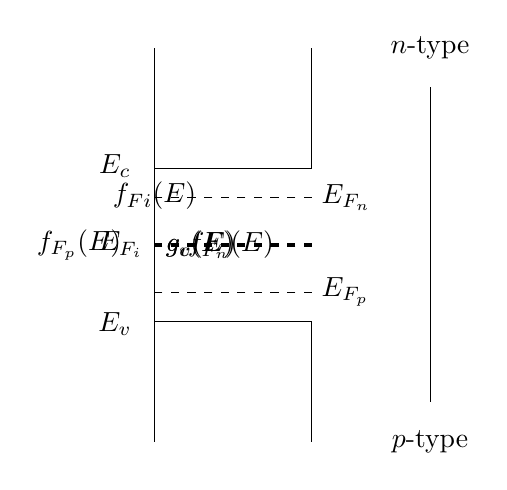
\begin{tikzpicture}
        \def\x{0.6}
        \draw[color=c2] (0,-2.5) -- ++(0,5) ++(2,0) -- ++(0,-1.525) -- ++(-2,0) ++(0,-1.95) -- ++(2,0) --++(0,-1.525);
        \draw[color=c2,ultra thick,dashed] (2,0) -- (0,0) node[left]{$E_{F_{i}}$};
        \draw[color=c2,dashed] (2,-\x) node[right]{$E_{F_p}$} -- (0,-\x);
        \draw[color=c2,dashed] (2,\x)  node[right]{$E_{F_n}$}--  (0,\x) ;
        \draw[domain=-2.2:2.2,smooth,dashed,color=c4,ultra thick] plot[parametric,id=band_gap_schematic_fermi] function{2/(1+exp((t)/0.5)),t} node[above=0.3cm ,sloped] {$f_{Fi}(E)$};
        \draw[domain=-2.2:2.2,smooth,dashed,color=c5] plot[parametric,id=band_gap_schematic_fermi] function{2/(1+exp((t-\x)/0.5)),t} node[right=0.3cm ,sloped] {$f_{F_n}(E)$};
        \draw[domain=-2.2:2.2,smooth,dashed,color=c7] plot[parametric,id=band_gap_schematic_fermi] function{2/(1+exp((t+\x)/0.5)),t} node[left=0.3cm ,sloped] {$f_{F_p}(E)$};
        \draw[domain=1:2,smooth, color=c5,ultra thick] plot[parametric,id=gc] function{2*(t-1)**0.5,t} node[right] {$g_c(E)$} ;
        \draw[domain=-1:-2,smooth, color=c7, ultra thick] plot[parametric,id=gv] function{2*(-1-t)**0.5,t} node[right] {$g_v(E)$} ;

        \draw[domain=1:2,smooth, color=c5] plot[parametric,id=gc] function{2/(1+exp((t-\x)/0.5))*2*(t-1)**0.5+3.5,t}     ;
        \draw[domain=-1:-2,smooth, color=c5] plot[parametric,id=gv] function{(2-2/(1+exp((t-\x)/0.5)))*2*(-1-t)**0.5+3.5,t} ;

        \draw[domain=1:2,smooth, color=c7] plot[parametric,id=gc] function{2/(1+exp((t+\x)/0.5))*2*(t-1)**0.5+3.5,t}     ;
        \draw[domain=-1:-2,smooth, color=c7] plot[parametric,id=gv] function{(2-2/(1+exp((t+\x)/0.5)))*2*(-1-t)**0.5+3.5,t} ;
        
        \draw[color=c2,ultra thin] (3.5,2) -- ++(0,-4);
        \node () at (-0.5,-1) {$E_v$};
        \node () at (-0.5,1) {$E_c$};
        \node[color=c5] () at (3.5,2.5) {$n$-type};
        \node[color=c7] () at (3.5,-2.5) {$p$-type};
%        \filldraw[fill=c5!60!white, draw=c5] (4,1.4) circle (0.5) node[above=\xcm,text width=2cm] { with $E_{F_n}$\\ donor};
%        \filldraw[fill=c5!60!white, draw=c5] (5.5,1.4) circle (0.2) node[above=\xcm,text width=2cm] { with $E_{F_n}$\\ acceptor};
%        \filldraw[fill=c7!60!white, draw=c7] (4,-1.4) circle (0.2); 
%        \filldraw[fill=c7!60!white, draw=c7] (5.5,-1.4) circle (0.5); 
       
\end{tikzpicture}
\end{document}

%pgfplots style picture
% comment tikzstyle figure out to get pgfplots style
\begin{document}
\begin{tikzpicture}
        \begin{axis}
                
        \end{axis}
\end{tikzpicture}
\end{document}

